% !TeX spellcheck = en_AU
% !TeX program = pdflatex
%
% LuxSleek-CV 1.1 LaTeX template
% Author: Andreï V. Kostyrka, University of Luxembourg
%
% 1.1: added tracking and letter-spacing for prettier lower caps, added `~` for language levels
% 1.0: initial release

\documentclass[11pt, a4paper]{article} 

\usepackage[T1]{fontenc}     % We are using pdfLaTeX,
\usepackage[utf8]{inputenc}  % hence this preparation
\usepackage[british]{babel}  
\usepackage[left = 0mm, right = 0mm, top = 0mm, bottom = 0mm]{geometry}
\usepackage[stretch = 25, shrink = 25, tracking=true, letterspace=30]{microtype}  
\usepackage{graphicx}        % To insert pictures
\usepackage{xcolor}          % To add colour to the document
\usepackage{marvosym}        % Provides icons for the contact details

\usepackage{enumitem}        % To redefine spacing in lists
\setlist{parsep = 0pt, topsep = 0pt, partopsep = 1pt, itemsep = 1pt, leftmargin = 6mm}

\usepackage{FiraSans}        % Change this to use any font, but keep it simple
\renewcommand{\familydefault}{\sfdefault}

\usepackage[most]{tcolorbox}

\definecolor{mybluei}{RGB}{124,156,205}
\definecolor{myblueii}{RGB}{73,121,193}
\definecolor{mygreen}{RGB}{202,217,126}
\definecolor{mypink}{RGB}{233,198,235}
\definecolor{myorange}{RGB}{255,127,80}
\definecolor{palegoldenrod}{RGB}{238,232,170}
\definecolor{darkpink}{RGB}{255, 155, 148}

\tcbset{
    innerbox/.style={fontupper=\sffamily\bfseries\small,
        size=small, colupper=white, halign=center, valign=center,
        colframe=white, boxrule=1pt, colback=mybluei},
    outerbox/.style={fontupper=\sffamily\bfseries,
        size=small, colupper=white, halign=center,
        colframe=black!70, boxrule=1pt, colback=myblueii, 
        boxsep=1pt, left=1pt, right=1pt},       
}

\definecolor{cvblue}{HTML}{304263}

\graphicspath{{./résumé}}

%%%%%%% USER COMMAND DEFINITIONS %%%%%%%%%%%%%%%%%%%%%%%%%%%
% These are the real workhorses of this template
\newcommand{\dates}[1]{\hfill\mbox{\textbf{#1}}} % Bold stuff that doesn’t got broken into lines
\newcommand{\is}{\par\vskip.5ex plus .4ex} % Item spacing
\newcommand{\smaller}[1]{{\small$\diamond$\ #1}}
\newcommand{\headleft}[1]{\vspace*{3ex}\textsc{\textbf{#1}}\par%
    \vspace*{-1.5ex}\hrulefill\par\vspace*{0.7ex}}
\newcommand{\headright}[1]{\vspace*{2.5ex}\textsc{\Large\color{cvblue}#1}\par%
     \vspace*{-2ex}{\color{cvblue}\hrulefill}\par}
%%%%%%%%%%%%%%%%%%%%%%%%%%%%%%%%%%%%%%%%%%%%%%%%%%%%%%%%%%%%

\usepackage[colorlinks = true, urlcolor = white, linkcolor = white]{hyperref}

\begin{document}

% Style definitions -- killing the unnecessary space and adding the skips explicitly
\setlength{\topskip}{0pt}
\setlength{\parindent}{0pt}
\setlength{\parskip}{0pt}
\setlength{\fboxsep}{0pt}
\pagestyle{empty}
\raggedbottom

\begin{minipage}[t]{0.33\textwidth} %% Left column -- outer definition
%  Left column -- top dark rectangle
\colorbox{cvblue}{\begin{minipage}[t][5mm][t]{\textwidth}\null\hfill\null\end{minipage}}

\vspace{-.2ex} % Eliminates the small gap
\colorbox{cvblue!90}{\color{white}  %% LEFT BOX
\kern0.09\textwidth\relax% Left margin provided explicitly
\begin{minipage}[t][293mm][t]{0.82\textwidth}
\raggedright
\vspace*{2.5ex}

\Large Samuel \textbf{\textsc{Marks}}, PhD \normalsize 

% Centering without extra vertical spacing
%\null\hfill\includegraphics[width=0.65\textwidth]{imagesuser.jpg}\hfill\null

\vspace*{0.5ex} % Extra space after the picture

\headleft{Modus Operandi}
Split my life in three: family; medical charity; and business. The unrelated-to-medicine business funds the first two. Focus is on open-source scalable engineering. Recently awarded an in-kind \textbf{grant worth \$3.2M} for neural compute processor access from Google.

\headleft{Links}
\small % To fit more content
\MVAt\ \href{mailto://samuelmarks@gmail.com}{\small samuelmarks@gmail.com} \\[0.4ex]
\Mundus\ \href{https://github.com/SamuelMarks}{github.com/SamuelMarks} \\[0.1ex]
\normalsize

\headleft{Career cliff notes}
\smaller{As a contractor working on unrelated sensor network metric aggregation, showed the largest communications company in Australia how to \textbf{save \$100M;}}\\
%   \item As a full-time employee at 16/17 years old, showed a large Travel
% company how to reduce staff count by 8 (making myself and my
% tech support department redundant);
\smaller{Given the entire top floor of the JP Morgan building to go from nothing to a full product in the Natural Language Processing (NLP) industry (all my subcontractors, including postdoctoral computational linguists)… with the backing of a billionaire family. Company \textbf{acquired by calendly};}\\
\smaller{Built a stock market analytics platform (for a high-net-worth individual);}\\
\smaller{Created deduplication algorithms and databases for helping one large bank\textemdash{}who bought another large bank\textemdash{}to join customer profiles (for a Venture Capital fund, who then proceeded to \textbf{raise \$60M} off this);}\\
\smaller{Engineered a distributed system for a blockchain company (my ‘stock’ in their company has since \textbf{gone up > 16000\%}).}

\end{minipage}%
\kern0.09\textwidth\relax%%Right margin provided explicitly to stretch the colourbox
}
\end{minipage}% Right column
\hskip2.5em% Left margin for the white area
\begin{minipage}[t]{0.56\textwidth}
\setlength{\parskip}{0.8ex}% Adds spaces between paragraphs; use \\ to add new lines without this space. Shrink this amount to fit more data vertically

\vspace{2ex}
\hypersetup{urlcolor=black}
\hypersetup{linkcolor=black}

\headright{Approach}
My goal is to develop open-source compilers, DevOps, and developer tooling in order to accelerate development, trivialise portability across platforms (OS; distribution; cloud), and facilitate onboarding of new engineers.

My current focus is engineering new compilers to [bidirectionally] translate OpenAPI \(\leftrightarrow\) numerous targets (including Rust, Swift, Kotlin Multiplatform, C, TypeScript, and Python) in order to speed up the development of multi-tier, multi-language applications (e.g., mobile apps; web frontends; REST API backends).

My recent work involved engineering new DevOps / GitOps / MLOps tooling where Docker is optional, with support for native Windows, Linux, macOS, SunOS, HP/UX, z/OS, iOS, and Android.  This was written in shell (Bourne Shell, Bash, Windows Batch, Microsoft PowerShell), complemented by new package managers in C, Go, and Rust.

I am research driven, holding a PhD and a fellowship at Harvard. I am a top contributor to Keras, the 2nd most popular Machine Learning framework. I have made C++ contributions to both PyTorch and TensorFlow for optimising their vector allocations. I am a Google Developer Expert for Machine Learnin (ML/AI GDE).

\headright{Technical expertise}
I take pride in working at every level of the stack:

\begin{tcbitemize}[raster columns=1, outerbox, 
    raster row skip=2pt]
    \tcbitem[colback=mybluei!40] 
        \begin{tcbitemize}[raster columns=6, raster rows=5, 
            raster equal height=all, 
            raster row skip=1pt, 
            raster column skip=1pt, 
            title style={left color=yellow!50!blue,right color=blue!50!green!50!black},
            innerbox]
            \tcbitem[raster multicolumn=6, colframe=blue!50!green!50!black, colback=blue!50!green!50!black, height=1cm] Stakeholders (users; customers; investors)
            \tcbitem Java (\mbox{Android})
            \tcbitem Swift (iOS)
            \tcbitem Kotlin Multiplatform (Android, iOS, web, desktop)
            \tcbitem Angular, HTML, SCSS (web)
            \tcbitem SDKs (C, Rust, go, Python, TypeScript, Kotlin, JavaScript)
            \tcbitem CLIs (cross-platform)
            \tcbitem[colback=myorange] Rust (actix + diesel)
            \tcbitem[colback=myorange] Python (Bottle; Flask; FastAPI)
            \tcbitem[raster multicolumn=2, colback=myorange] (Node.js; Bun; Deno) with (TypeScript + ORMs + express \textbar{} restify)
            \tcbitem[colback=myorange] go
            \tcbitem[colback=myorange] C/C++
            \tcbitem[colback=purple]Build systems (CMake, Makefile, Fabric; clang, vcpkg)
            \tcbitem[raster multicolumn=2, colback=purple] Package management (incl. package authoring; and new package managers)
            \tcbitem[raster multicolumn=2, colback=purple] Multicloud (Apache Libcloud contrib. 30+ clouds incl. AWS, Google Cloud, VMware, \textellipsis{})
            \tcbitem[colback=purple] Cross-platform deployment shell scripts
            \tcbitem[raster multicolumn=3,colback=darkpink] TensorFlow, PyTorch, Keras, MaxText (large-scale LLM training) contributions
            \tcbitem[raster multicolumn=3, colback=mygreen!140] Compilers to go from/to OpenAPI
        \end{tcbitemize}
%    \tcbitem[colback=myblueii, height=8mm, valign=center] Java Runtime
\end{tcbitemize}

\headright{Experience}

\textit{Mass. Eye and Ear Infirmary / Harvard Medical School.}  \dates{2021+} \\
\smaller{Collaborating with ophthalmologists on initiating new medical diagnostic screening programmes that are wholly charitable, open-source, patent-free, and AI-driven; and analysing \& modelling from historical data in preparation.}

\is
\textsc{Head of software engineering} at \textit{consultancy \href{https://offscale.io}{offscale.io}} \dates{2015+} \\
\smaller{Consulting for various high-net-worth individuals, the odd venture capital firm, and any random project introduced word-of-mouth to me. Ranges from just me, to as many as 20 engineers.}

\smaller{Engineers open-source developer tools to speedup engineering of scalable software. Foci on: cross-platform, multi-ML, multicloud, and compilers to translate across codebases. \href{https://github.com/offscale}{github.com/offscale}}

\smaller{\textit{NOTE: Firm purposefully avoids anything related to medicine to avoid actual\textemdash{}or perceived\textemdash{}conflicts of interest with charitable research.}} 


\headright{Education}

\textsc{Fellowship}. \textit{Harvard Medical School}. \dates{2021+}

\textsc{Doctor of Philosophy (PhD)}. \textit{University of Sydney}. \dates{2015--2020}

\is
\textsc{Bachelor of Science}. School of Computing. \textit{Macquarie U}.  \dates{2010--2014}
\smaller{Covered a range of subjects supporting my passion for computer science.}


\headright{Open-source}

700+ repositories on GitHub, >300 of these original projects (not forks). Top-10 contributor to Google's Keras (2nd-most popular ML framework; with 13 million downloads per month; as of Feb 2025).

\end{minipage}

\begin{minipage}[t]{0.33\textwidth} %% Left column -- outer definition
%  Left column -- top dark rectangle
\colorbox{cvblue}{\begin{minipage}[t][5mm][t]{\textwidth}\null\hfill\null\end{minipage}}

\vspace{-.2ex} % Eliminates the small gap
\colorbox{cvblue!90}{\color{white}  %% LEFT BOX
\kern0.09\textwidth\relax% Left margin provided explicitly
\begin{minipage}[t][293mm][t]{0.82\textwidth}
\raggedright
\vspace*{2.5ex}

\Large Samuel \textbf{\textsc{Marks}}, PhD \normalsize 

% Centering without extra vertical spacing
%\null\hfill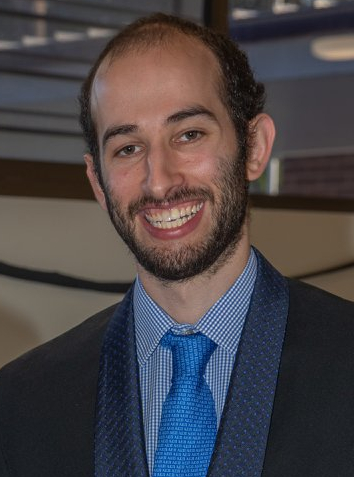
\includegraphics[width=0.65\textwidth]{user.jpg}\hfill\null

\vspace*{0.5ex} % Extra space after the picture

\headleft{Differentiator}
I build technologies to speed-up development, and futureproof software-engineering.

\headleft{Links}
\small % To fit more content
\MVAt\ \href{mailto://samuelmarks@gmail.com}{\small samuelmarks@gmail.com} \\[0.4ex]
\Mundus\ \href{https://github.com/SamuelMarks}{github.com/SamuelMarks} \\[0.1ex]
\normalsize

\headleft{Open source projects}
800+ GitHub repositories, incl.:\\
\smaller{Compiler implementations in Rust, Python, C, Swift, Java, and Kotlin}\\
\smaller{OAuth2 server implementations in Rust, Python, and Node.js}\\
\smaller{New package managers in: go; Bourne Shell (\texttt{/bin/sh}); C; and Rust}\\
\smaller{Getting-started scaffolds in Angular, Python, Rust, Swift, Kotlin, Java}\\
\smaller{\textbraceleft{}CLI, SQL, GUI, SDK\textbraceright{} [bidirectional] generation from/to Python SDKs, e.g., major machine-learning frameworks like Keras}\\
\smaller{Multicloud provisioning and deprovisioning toolchains, including new JSON wrappers in Python, a new Google Cloud C SDK, and a new WASM implementation}\\
\smaller{1-click deployment + documentation system generation from my new shell script library; including porting Apache Libcloud to WASM (WebAssembly)}

\end{minipage}%
\kern0.09\textwidth\relax%%Right margin provided explicitly to stretch the colourbox
}
\end{minipage}% Right column
\hskip2.5em% Left margin for the white area
\begin{minipage}[t]{0.56\textwidth}
\setlength{\parskip}{0.8ex}% Adds spaces between paragraphs; use \\ to add new lines without this space. Shrink this amount to fit more data vertically

\vspace{2ex}
\hypersetup{urlcolor=black}
\hypersetup{linkcolor=black}

\headright{Experience}

\textit{Mass. Eye and Ear Infirmary / Harvard Medical School.}  \dates{2021+} \\
\smaller{Collaborating with ophthalmologists on initiating new medical diagnostic screening programmes that are wholly charitable, open-source, patent-free, and AI-driven; and analysing \& modelling from historical data in preparation.}

\is
\textsc{Head of software engineering} at \textit{consultancy \href{https://offscale.io}{offscale.io}} \dates{2015+} \\
\smaller{Consulting for various high-net-worth individuals, the odd venture capital firm, and any random project introduced word-of-mouth to me. Ranges from just me, to as many as 20 engineers.}

\smaller{Engineers open-source developer tools to speedup engineering of scalable software. Foci on: cross-platform, multi-ML, multicloud, and compilers to translate across codebases. \href{https://github.com/offscale}{github.com/offscale}}

\smaller{\textit{NOTE: Firm purposefully avoids anything related to medicine to avoid actual\textemdash{}or perceived\textemdash{}conflicts of interest with charitable research.}} 


\headright{Education}

\textsc{Fellowship}. \textit{Harvard Medical School}. \dates{2021+}

\textsc{Doctor of Philosophy (PhD)}. \textit{University of Sydney}. \dates{2015--2020}

\is
\textsc{Bachelor of Science}. School of Computing. \textit{Macquarie U}.  \dates{2010--2014}
\smaller{Covered a range of subjects supporting my passion for computer science.}


\headright{Open-source}
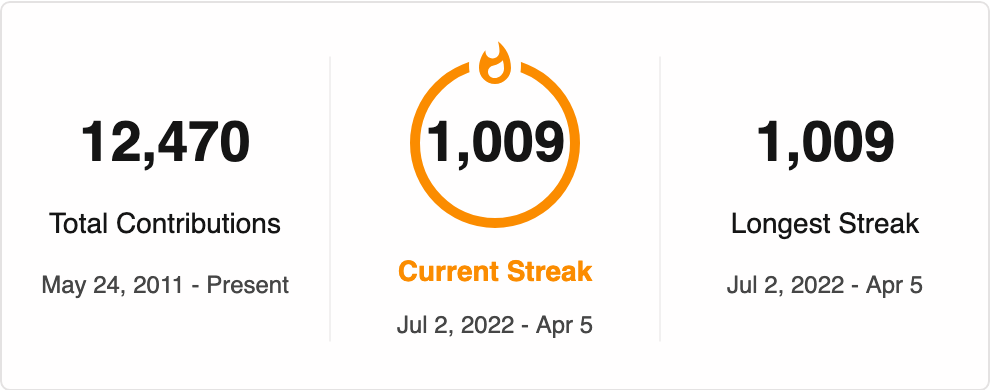
\includegraphics[width=1.101\columnwidth]{images/github0.png}
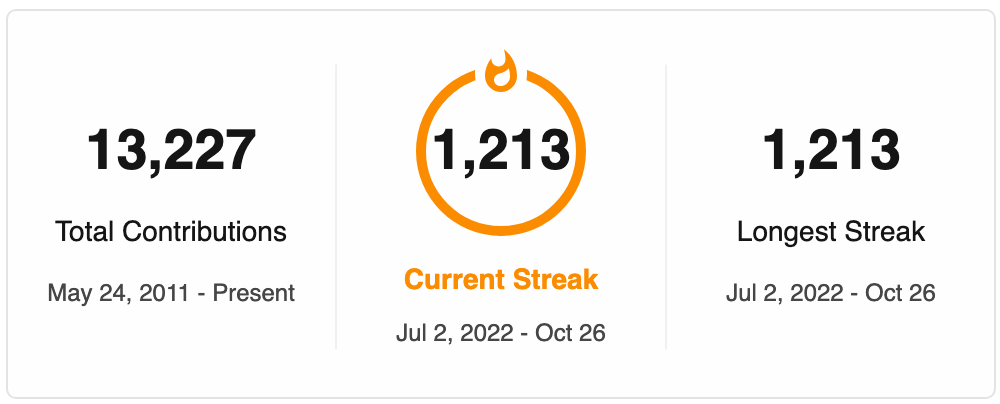
\includegraphics[width=1.101\columnwidth]{images/github1.png}
800+ repositories on GitHub, >300 of these original projects (not forks). Top-10 contributor to Google's \href{https://keras.io}{Keras} (2nd-most popular ML framework; with 13 million downloads per month; as of Feb 2025). Only non-Google maintainer of Google's large-scale LLM training reference\textemdash{}that they test on >50,000 TPUs\textemdash{}\href{https://github.com/AI-Hypercomputer/maxtext}{https://github.com/AI-Hypercomputer/maxtext}.

\end{minipage}

\end{document}
